% ============================================================
% LAPORAN PRAKTIKUM ALGORITMA DAN PEMROGRAMAN
% Modul 3 & 4: Pola Perulangan: Penelusuran, Penanda, dan Pengolahan Data
% Compile dengan pdfLaTeX
% ============================================================

\documentclass[12pt,a4paper]{article}

% ---------- Font sederhana ----------
\usepackage[T1]{fontenc}
\usepackage[utf8]{inputenc}
\usepackage{mathptmx}

% ---------- Tata letak ----------
\usepackage[a4paper,left=3cm,right=2cm,top=2cm,bottom=2cm]{geometry}
\usepackage{setspace}
\setstretch{1.15}
\usepackage{ragged2e}
\justifying
\setlength{\parindent}{1.25cm}
\setlength{\parskip}{0pt}

% ---------- Paket umum ----------
\usepackage{graphicx}
\usepackage{float}
\usepackage{enumitem}
\usepackage{titlesec}
\usepackage{array}
\usepackage{booktabs}
\usepackage{longtable}
\usepackage{caption}
\usepackage{hyperref}
\usepackage{amsmath}
\hypersetup{hidelinks}

% ---------- Format heading ----------
\titleformat{\section}
  {\bfseries\fontsize{12pt}{14pt}\selectfont}
  {}{0pt}{}
\titlespacing*{\section}{0pt}{12pt}{6pt}

\titleformat{\subsection}
  {\bfseries\fontsize{12pt}{14pt}\selectfont}
  {}{0pt}{}
\titlespacing*{\subsection}{0pt}{10pt}{4pt}

\titleformat{\subsubsection}
  {\bfseries\fontsize{12pt}{14pt}\selectfont}
  {}{0pt}{}
\titlespacing*{\subsubsection}{0pt}{8pt}{3pt}

\setlist[enumerate]{leftmargin=1.1cm,itemsep=0pt,topsep=2pt}
\setlist[itemize]{leftmargin=1.1cm,itemsep=0pt,topsep=2pt}

% ---------- Helper template ----------
\newcommand{\placeholder}[1]{\textit{[#1]}}
\newcommand{\imageplaceholder}[1]{%
  \begin{center}
  \fbox{\parbox[c][5.5cm][c]{0.88\textwidth}{\centering\textit{[#1]}}}
  \end{center}
}

\begin{document}

% ============================================================
% COVER
% ============================================================
\begin{titlepage}
\thispagestyle{empty}
\begin{center}

{\bfseries\fontsize{16pt}{19pt}\selectfont LAPORAN PRAKTIKUM\par}
\vspace{0.25cm}
{\bfseries\fontsize{16pt}{19pt}\selectfont ALGORITMA DAN PEMROGRAMAN\par}
\vspace{0.45cm}
{\bfseries\fontsize{14pt}{17pt}\selectfont MODUL 3 \& 4\par}
\vspace{0.15cm}
{\bfseries\fontsize{14pt}{17pt}\selectfont POLA PERULANGAN: PENELUSURAN, PENANDA, DAN PENGOLAHAN DATA\par}

\vspace{1.2cm}

\IfFileExists{logo_telkom_university.png}{%
  
\includegraphics[width=0.34\textwidth]{logo_telkom_university.png}%
}{%
  \IfFileExists{../logo_telkom_university.png}{%
    \includegraphics[width=0.34\textwidth]{../logo_telkom_university.png}%
  }{%
    \IfFileExists{../../logo_telkom_university.png}{%
      
\includegraphics[width=0.34\textwidth]{../../logo_telkom_university.png}%
    }{%
      \fbox{\parbox[c][3.5cm][c]{0.34\textwidth}{\centering\textit{[Logo Telkom University]}}}%
    }%
  }%
}

\vspace{1.2cm}

\renewcommand{\arraystretch}{1.35}
\begin{tabular}{>{\bfseries}p{2.3cm} p{0.35cm} p{8.4cm}}
NAMA  & : & DENDRA DE TAMA \\
NIM   & : & 108052600034 \\
KELAS & : & SS1SI-50-REG-01 \\
PRODI & : & S1 SISTEM INFORMASI \\
\end{tabular}

\vfill

{\bfseries TELKOM UNIVERSITY SURABAYA\par}
{\bfseries FAKULTAS REKAYASA INDUSTRI\par}
{\bfseries PROGRAM STUDI S1 SISTEM INFORMASI\par}
\vspace{0.2cm}
{\bfseries TAHUN AKADEMIK 2025/2026\par}

\end{center}
\end{titlepage}

% ============================================================
% PENDAHULUAN
% ============================================================
\section{PENDAHULUAN}
Perulangan merupakan salah satu mekanisme paling mendasar dan krusial dalam pemrograman terstruktur. Namun, implementasi perulangan dalam rekayasa perangkat lunak tidak hanya menuntut kode yang dapat berjalan (*executable*), melainkan kode yang terbukti deterministik, bebas galat logika batas (*boundary error*), dan memiliki ketahanan (*robustness*) terhadap anomali data masukan. Modul Praktikum 3 dan 4 mengonsolidasikan prinsip-prinsip perancangan dan verifikasi perulangan tingkat menengah pada bahasa Python 3 melalui paradigma pengolahan data terstruktur.

Aspek pertama yang menjadi landasan utama adalah teknik penelusuran status perulangan (*loop state tracing*) dan pembuktian jaminan berhenti (*termination guarantee*). Dengan memanfaatkan tabel penelusuran (*trace table*), transisi nilai dari variabel kendali putaran dan variabel penampung (*state variables*) dapat dipantau di setiap langkah komputasi. Penelusuran ini secara efektif mendeteksi dan mencegah kesalahan klasik satu putaran (*off-by-one error* / OBOE), seperti ketidaktepatan dalam memilih operator relasional batas ($\le$ versus $<$) serta pengujian ketahanan program pada kondisi ekstrem ($n = 0$ dan $n = 1$).

Aspek kedua berfokus pada arsitektur masukan berpenanda (*sentinel-controlled loop*). Berbeda dengan perulangan terhitung yang telah mengetahui kuantitas data di awal, skema penanda memungkinkan pembacaan data dinamis yang diakhiri oleh suatu nilai khusus (seperti $-1$ atau $0$). Penerapan pola baca ganda (*read-twice pattern*), yaitu pembacaan inisiasi sebelum perulangan (*priming read*) dan pembacaan pembaruan di akhir badan perulangan (*update read*), menjadi keharusan mutlak agar nilai penanda tidak mengontaminasi akumulator atau pencacah data. Selain itu, proteksi pembagian nol (*zero-division guard*) mutlak disematkan guna menangani kemungkinan pengguna langsung menghentikan program tanpa memasukkan data riil.

Aspek ketiga mencakup integrasi pola-pola komputasi lanjut dalam pengolahan deret data:
\begin{enumerate}
    \item \textbf{Pola Akumulator (\textit{Accumulator Pattern}) dan Pencacah (\textit{Counter Pattern})}: Menghitung jumlahan parsial skalar dan frekuensi keterjadian kondisi tertentu secara simultan.
    \item \textbf{Pola Penyaringan (\textit{Filtering Pattern})}: Memisahkan subset data yang memenuhi kriteria ambang batas (\textit{threshold}) dari deret data agregat untuk analisis selektif.
    \item \textbf{Pelacakan Nilai Ekstrem (\textit{Extremum Tracking}) dan Jebakan Inisialisasi}: Menentukan nilai maksimum dan minimum secara berkesinambungan. Kesalahan umum menginisialisasi nilai awal dengan angka nol ($tertinggi = 0$) berakibat fatal ketika seluruh data bernilai negatif. Modul ini mengajarkan pola penanda \texttt{None} atau pola inisialisasi rekaman pertama (*first-record initialization*) untuk menjamin akurasi absolut, disertai pelacakan indeks temporal terjadinya nilai ekstrem (*temporal/index tracking*).
    \item \textbf{Dekomposisi dan Pengelompokan Masalah (\textit{Problem Grouping})}: Menguraikan permasalahan kompleks menjadi sub-masalah modular dengan pola algoritmik independen sebelum diintegrasikan ke dalam satu alur kendali.
\end{enumerate}

Laporan praktikum terpadu ini menyajikan evaluasi terhadap delapan rancangan program: empat latihan penelusuran dan batas deret dari Modul 3 (\texttt{latihan1.py} s.d. \texttt{latihan4.py} Week 3), tiga latihan lanjutan penyaringan, jebakan inisialisasi, dan pengelompokan masalah dari Modul 4 (\texttt{latihan1.py} s.d. \texttt{latihan3.py} Week 4), serta satu studi kasus komprehensif sistem rekapitulasi lini perakitan pabrik (\texttt{studi\_kasus.py}).

\subsection{Tujuan Praktikum}
\begin{enumerate}
    \item Memahami dan menyusun tabel penelusuran (\textit{trace table}) untuk memverifikasi transisi state, invarian perulangan, dan jaminan terminasi program.
    \item Menganalisis, merekonstruksi, dan mencegah kesalahan batas satu putaran (\textit{off-by-one error}) serta menguji ketahanan program pada kasus batas ($n=0$, $n=1$).
    \item Menerapkan pola perulangan berpenanda (*sentinel*) dengan skema baca ganda (*read-twice pattern*) dan proteksi pembagian dengan nol (*zero-division guard*).
    \item Menguasai integrasi pola akumulator, pencacah kondisional, dan penyaringan ambang batas (*conditional filtering*).
    \item Memahami bahaya jebakan inisialisasi nilai ekstrem (*initial value pitfall*) pada domain data negatif serta menerapkan solusi berbasis penanda \texttt{None} dan inisialisasi rekaman pertama.
    \item Menerapkan teknik pengelompokan masalah (*problem grouping*) dan pelacakan indeks kejadian ekstrem dalam menyelesaikan persoalan rekapitulasi data multidimensi.
\end{enumerate}

% ============================================================
% LANGKAH PERCOBAAN
% ============================================================
\section{LANGKAH--LANGKAH PERCOBAAN}

\subsection{Percobaan 1: Penelusuran Perulangan While dan Tabel Trace (Week 3 - latihan1.py)}
\begin{enumerate}
    \item Pemahaman Persoalan: Program menghitung akumulasi penjumlahan bilangan kelipatan dua dari interval $n = 1$ hingga $n = 5$ menggunakan struktur \texttt{while}. Tujuan utama latihan ini adalah melakukan verifikasi kebenaran logika melalui penelusuran manual tabel *trace* terhadap variabel akumulator \texttt{total} dan variabel langkah \texttt{n}.
    \item Data Masukan/Keluaran:
    \begin{itemize}
        \item Masukan: Tidak ada masukan dinamis konsol (nilai awal $total=0$ dan $n=1$ diinisialisasi pada kode sumber).
        \item Keluaran: Teks konfirmasi nilai akumulasi akhir: \texttt{total = 30}.
    \end{itemize}
    \item Penyusunan Algoritma:
    \begin{enumerate}[label=\alph*.]
        \item Mulai program.
        \item Inisialisasi variabel akumulator $total = 0$ dan pencacah $n = 1$.
        \item Uji kondisi perulangan: selama $n \le 5$:
        \begin{enumerate}[label=\roman*.]
            \item Tambahkan nilai $n \times 2$ ke dalam variabel \texttt{total}: $total = total + n \times 2$.
            \item Tambahkan nilai variabel langkah: $n = n + 1$.
        \end{enumerate}
        \item Cetak string \texttt{"total ="} diikuti nilai akhir variabel \texttt{total}.
        \item Selesai.
    \end{enumerate}
\end{enumerate}

\subsection{Percobaan 2: Analisis Kesalahan Off-by-One pada Penjumlahan Deret (Week 3 - latihan2.py)}
\begin{enumerate}
    \item Pemahaman Persoalan: Program bertugas menjumlahkan deret bilangan bulat berurutan dari 1 sampai $n$. Program ini dirancang untuk menguji batas inklusifitas iterasi ($i \le n$ versus $i < n$) guna mencegah hilangnya angka terakhir deret (*off-by-one error*), serta menjamin stabilitas ketika pengguna menginputkan nilai batas nol ($n = 0$).
    \item Data Masukan/Keluaran:
    \begin{itemize}
        \item Masukan: Sebuah bilangan bulat non-negatif $n$ (integer).
        \item Keluaran: Kalimat penetapan hasil penjumlahan total: \texttt{Jumlah: [total]}.
    \end{itemize}
    \item Penyusunan Algoritma:
    \begin{enumerate}[label=\alph*.]
        \item Mulai program.
        \item Minta masukan nilai batas atas dari pengguna dan simpan ke variabel integer \texttt{n}.
        \item Inisialisasi variabel akumulator $total = 0$ dan variabel iterasi $i = 1$.
        \item Uji kondisi perulangan inklusif: selama $i \le n$:
        \begin{enumerate}[label=\roman*.]
            \item Akumulasikan nilai: $total = total + i$.
            \item Perbarui variabel langkah: $i = i + 1$.
        \end{enumerate}
        \item Tampilkan hasil perhitungan: \texttt{"Jumlah:", total}.
        \item Selesai.
    \end{enumerate}
\end{enumerate}

\subsection{Percobaan 3: Perulangan Sentinel dan Proteksi Pembagian Nol (Week 3 - latihan3.py)}
\begin{enumerate}
    \item Pemahaman Persoalan: Program menghitung nilai rata-rata durasi waktu proses mesin dalam satuan menit. Karena banyaknya pencatatan tidak terikat kuantitas pasti, penghentian iterasi dikendalikan oleh nilai penanda (*sentinel*) $-1$. Program mengimplementasikan pola baca ganda (*read-twice pattern*) agar nilai $-1$ tidak dihitung sebagai data durasi, serta menyertakan percabangan pelindung pembagian nol (*zero-division guard*) jika pengguna tidak memasukkan data sama sekali.
    \item Data Masukan/Keluaran:
    \begin{itemize}
        \item Masukan: Serangkaian bilangan bulat durasi waktu proses (menit) yang diakhiri dengan angka $-1$.
        \item Keluaran: Banyaknya data yang dimasukkan beserta rata-rata durasi berpresisi dua angka di belakang koma, atau pesan \texttt{"Belum ada data yang dimasukkan."} jika data kosong.
    \end{itemize}
    \item Penyusunan Algoritma:
    \begin{enumerate}[label=\alph*.]
        \item Mulai program.
        \item Inisialisasi variabel $total = 0$ dan $banyak = 0$.
        \item Lakukan pembacaan data awal (*priming read*): baca masukan durasi pengguna ke variabel \texttt{durasi}.
        \item Uji kondisi sentinel: selama $durasi \ne -1$:
        \begin{enumerate}[label=\roman*.]
            \item Akumulasikan durasi: $total = total + durasi$.
            \item Tambahkan pencacah data: $banyak = banyak + 1$.
            \item Lakukan pembacaan data berikutnya (*loop-end read*): baca kembali ke variabel \texttt{durasi}.
        \end{enumerate}
        \item Uji validitas keberadaan data: jika $banyak == 0$:
        \begin{itemize}
            \item Cetak pesan konfirmasi: \texttt{"Belum ada data yang dimasukkan."}.
        \end{itemize}
        \item Selain itu ($banyak > 0$):
        \begin{itemize}
            \item Cetak teks \texttt{"Banyak data:"} diikuti nilai \texttt{banyak}.
            \item Hitung rata-rata dengan pembulatan dua desimal: $\text{round}(total / banyak, 2)$ dan tampilkan hasilnya.
        \end{itemize}
        \item Selesai.
    \end{enumerate}
\end{enumerate}

\subsection{Percobaan 4: Pola Akumulator dan Pencacah Produksi Harian (Week 3 - latihan4.py)}
\begin{enumerate}
    \item Pemahaman Persoalan: Program merekapitulasi data volume produksi harian pabrik selama periode konstan 10 hari. Target produksi harian ditetapkan pada konstanta 50 unit. Program menerapkan pola akumulator untuk menghitung total produksi, menghitung rata-rata harian, serta menerapkan pola pencacah bersyarat untuk menghitung frekuensi hari kerja di mana produksi tidak mencapai target ($< 50$).
    \item Data Masukan/Keluaran:
    \begin{itemize}
        \item Masukan: Sepuluh bilangan bulat integer yang merepresentasikan angka produksi hari ke-1 sampai hari ke-10.
        \item Keluaran: Tiga baris ringkasan: total produksi keseluruhan, rata-rata produksi harian, dan jumlah hari produksi di bawah target.
    \end{itemize}
    \item Penyusunan Algoritma:
    \begin{enumerate}[label=\alph*.]
        \item Mulai program.
        \item Tetapkan konstanta ambang: $TARGET = 50$ dan durasi: $HARI = 10$.
        \item Inisialisasi variabel: $total = 0$ dan $di\_bawah = 0$.
        \item Lakukan perulangan \texttt{for} dengan variabel \texttt{hari} pada rentang \texttt{range(1, HARI + 1)}:
        \begin{enumerate}[label=\roman*.]
            \item Baca masukan produksi harian ke variabel \texttt{produksi}.
            \item Akumulasikan ke total: $total = total + produksi$.
            \item Uji kondisi ambang batas: jika $produksi < TARGET$, maka tambahkan pencacah $di\_bawah = di\_bawah + 1$.
        \end{enumerate}
        \item Cetak informasi total produksi: \texttt{"Total produksi:", total}.
        \item Hitung dan cetak rata-rata: \texttt{"Rata-rata per hari:", total / HARI}.
        \item Cetak frekuensi hari di bawah target: \texttt{"Hari di bawah target:", di\_bawah}.
        \item Selesai.
    \end{enumerate}
\end{enumerate}

\subsection{Percobaan 5: Pola Penyaringan Produksi Terhadap Target (Week 4 - latihan1.py)}
\begin{enumerate}
    \item Pemahaman Persoalan: Program berfungsi sebagai sistem penyaring (*filtering pattern*) produksi selama 10 hari terhadap ambang target $TARGET = 50$. Berbeda dengan akumulasi total biasa, program hanya mengagregasikan unit produksi pada hari-hari yang berhasil mencapai atau melampaui target ($\ge 50$), menghitung berapa hari yang lolos, serta menghitung rata-rata khusus hari lolos target dengan proteksi jika tidak ada satupun hari yang mencapai target.
    \item Data Masukan/Keluaran:
    \begin{itemize}
        \item Masukan: Sepuluh bilangan bulat produksi harian (hari ke-1 sampai ke-10).
        \item Keluaran: Banyaknya hari yang mencapai target, total unit produksi yang dihasilkan pada hari-hari tersebut, dan rata-rata unit harian khusus hari lolos target, atau pesan pemberitahuan khusus bila tidak ada hari yang lolos.
    \end{itemize}
    \item Penyusunan Algoritma:
    \begin{enumerate}[label=\alph*.]
        \item Mulai program.
        \item Inisialisasi konstanta: $TARGET = 50$ dan $HARI = 10$.
        \item Inisialisasi akumulator penyaring: $total\_lolos = 0$ dan $banyak\_lolos = 0$.
        \item Lakukan perulangan \texttt{for} dengan variabel \texttt{hari} dari 1 sampai $HARI$:
        \begin{enumerate}[label=\roman*.]
            \item Baca data produksi ke variabel \texttt{produksi}.
            \item Uji penyaring: jika $produksi \ge TARGET$:
            \begin{itemize}
                \item Akumulasikan nilai: $total\_lolos = total\_lolos + produksi$.
                \item Tambahkan pencacah: $banyak\_lolos = banyak\_lolos + 1$.
            \end{itemize}
        \end{enumerate}
        \item Uji kondisi ketiadaan data lolos: jika $banyak\_lolos == 0$:
        \begin{itemize}
            \item Cetak kalimat: \texttt{"Tidak ada hari yang mencapai target."}.
        \end{itemize}
        \item Selain itu ($banyak\_lolos > 0$):
        \begin{itemize}
            \item Hitung rata-rata data lolos: $rata = \text{round}(total\_lolos / banyak\_lolos, 2)$.
            \item Tampilkan banyak hari mencapai target, total unit, dan nilai rata-rata unit tersebut.
        \end{itemize}
        \item Selesai.
    \end{enumerate}
\end{enumerate}

\subsection{Percobaan 6: Pelacakan Nilai Ekstrem dan Jebakan Inisialisasi (Week 4 - latihan2.py)}
\begin{enumerate}
    \item Pemahaman Persoalan: Program mencatat nilai laba bersih bulanan perusahaan selama semester pertama (6 bulan) dan mencari laba tertinggi beserta urutan bulan terjadinya. Latihan ini secara khusus menyoroti bahaya kesalahan perancangan nilai awal (*initial value pitfall*), di mana inisialisasi $tertinggi = 0$ akan menghasilkan kesimpulan yang salah apabila seluruh bulan mengalami defisit/laba negatif. Pola inisialisasi yang diterapkan adalah menggunakan nilai sentinel \texttt{None}.
    \item Data Masukan/Keluaran:
    \begin{itemize}
        \item Masukan: Enam nilai laba bersih bulanan bertipe integer (dalam satuan juta rupiah).
        \item Keluaran: Informasi nilai laba tertinggi yang tercapai beserta nomor bulan spesifik di mana laba tersebut dibukukan.
    \end{itemize}
    \item Penyusunan Algoritma:
    \begin{enumerate}[label=\alph*.]
        \item Mulai program.
        \item Inisialisasi penanda ekstrem: tetapkan $tertinggi = \text{None}$ dan $bulan\_tertinggi = \text{None}$.
        \item Lakukan perulangan \texttt{for} dengan variabel \texttt{bulan} pada rentang \texttt{range(1, 7)}:
        \begin{enumerate}[label=\roman*.]
            \item Baca masukan laba bulanan ke variabel \texttt{laba}.
            \item Uji pembaruan ekstrem: jika $tertinggi \text{ is None}$ atau $laba > tertinggi$:
            \begin{itemize}
                \item Perbarui nilai tertinggi: $tertinggi = laba$.
                \item Simpan indeks temporal: $bulan\_tertinggi = bulan$.
            \end{itemize}
        \end{enumerate}
        \item Tampilkan hasil evaluasi laba maksimum menggunakan pemformatan f-string: \texttt{f"Laba tertinggi: \{tertinggi\} juta (bulan ke-\{bulan\_tertinggi\})"}.
        \item Selesai.
    \end{enumerate}
\end{enumerate}

\subsection{Percobaan 7: Pengelompokan Masalah Suhu Mesin (Week 4 - latihan3.py)}
\begin{enumerate}
    \item Pemahaman Persoalan: Program memproses delapan kali pencatatan suhu sensor mesin industri secara berkala. Program menerapkan teknik rekayasa dekomposisi masalah (*problem grouping*) dengan memecah instruksi menjadi tiga sub-masalah fungsional: (1) pelacakan suhu tertinggi dan waktu pencatatan ke berapa, (2) pencacahan berapa kali suhu melewati batas bahaya ($> 80^\circ\text{C}$), serta (3) perhitungan rata-rata suhu yang berada di atas ambang bahaya tersebut.
    \item Data Masukan/Keluaran:
    \begin{itemize}
        \item Masukan: Delapan bilangan bulat data suhu sensor mesin (ke-1 sampai ke-8).
        \item Keluaran: Nilai suhu tertinggi beserta nomor urutnya, frekuensi kejadian suhu melebihi $80^\circ$, serta nilai rata-rata suhu yang berada di atas ambang tersebut dengan format dua digit desimal.
    \end{itemize}
    \item Penyusunan Algoritma:
    \begin{enumerate}[label=\alph*.]
        \item Mulai program.
        \item Inisialisasi variabel dari ketiga sub-masalah:
        \begin{itemize}
            \item Sub-masalah 1: $tertinggi = \text{None}$, $urutan\_tertinggi = \text{None}$.
            \item Sub-masalah 2: $banyak\_diatas\_80 = 0$.
            \item Sub-masalah 3: $total\_diatas\_80 = 0$.
        \end{itemize}
        \item Lakukan perulangan \texttt{for} dengan indeks $i$ dari 1 hingga 8:
        \begin{enumerate}[label=\roman*.]
            \item Baca nilai suhu ke variabel \texttt{suhu}.
            \item Evaluasi sub-masalah 1: jika $tertinggi \text{ is None}$ atau $suhu > tertinggi$: perbarui $tertinggi = suhu$ dan $urutan\_tertinggi = i$.
            \item Evaluasi sub-masalah 2 dan 3: jika $suhu > 80$: perbarui $banyak\_diatas\_80 = banyak\_diatas\_80 + 1$ dan $total\_diatas\_80 = total\_diatas\_80 + suhu$.
        \end{enumerate}
        \item Cetak informasi suhu tertinggi dan urutan pencatatannya.
        \item Uji ketersediaan data di atas $80^\circ$: jika $banyak\_diatas\_80 == 0$, tampilkan \texttt{"Tidak ada suhu yang melebihi 80"}. Selain itu, hitung rata-rata $rata\_rata = total\_diatas\_80 / banyak\_diatas\_80$ dan cetak dengan presisi \texttt{.2f}.
        \item Selesai.
    \end{enumerate}
\end{enumerate}

\subsection{Percobaan 8: Studi Kasus Rekapitulasi Produksi Lini Perakitan (Week 4 - studi\_kasus.py)}
\begin{enumerate}
    \item Pemahaman Persoalan: Program mengimplementasikan sistem rekapitulasi data produksi lini perakitan pabrik berskala penuh yang memadukan seluruh pola perulangan: pembacaan berpenanda sentinel $-1$, pelacakan nilai ekstrem (tertinggi dan terendah) dengan aturan penentu hari terawal saat terjadi nilai kembar (*earliest tie-breaker*), perhitungan statistik menyeluruh (banyak hari, total produksi, dan rata-rata per hari), penyaringan hari pemenuhan target harian ($\ge 100$), serta penyelesaian tantangan rata-rata produksi khusus hari target.
    \item Data Masukan/Keluaran:
    \begin{itemize}
        \item Masukan: Rangkaian volume produksi harian yang diinputkan pengguna secara interaktif hingga diakhiri dengan angka $-1$.
        \item Keluaran: Laporan rekapitulasi komprehensif mencakup banyak hari kerja, total akumulasi produksi, rata-rata harian, hari pemenuhan target, capaian tertinggi beserta harinya, capaian terendah beserta harinya, serta rata-rata khusus hari target.
    \end{itemize}
    \item Penyusunan Algoritma:
    \begin{enumerate}[label=\alph*.]
        \item Mulai program.
        \item Deklarasikan konstanta: $TARGET = 100$ dan $PENANDA = -1$.
        \item Inisialisasi variabel statistik: $banyak\_hari = 0$, $total\_produksi = 0$, $hari\_target = 0$, $total\_target = 0$, serta penanda ekstrem: $tertinggi = \text{None}$, $hari\_tertinggi = \text{None}$, $terendah = \text{None}$, $hari\_terendah = \text{None}$.
        \item Lakukan pembacaan awal masukan produksi hari ke-1 ke variabel \texttt{produksi}.
        \item Jalankan perulangan \texttt{while} dengan kondisi $produksi \ne PENANDA$:
        \begin{enumerate}[label=\roman*.]
            \item Tambahkan pencacah hari: $banyak\_hari = banyak\_hari + 1$.
            \item Tambahkan akumulasi total: $total\_produksi = total\_produksi + produksi$.
            \item Pengujian rekaman pertama: jika $banyak\_hari == 1$:
            \begin{itemize}
                \item Tetapkan $tertinggi = produksi$, $hari\_tertinggi = 1$.
                \item Tetapkan $terendah = produksi$, $hari\_terendah = 1$.
            \end{itemize}
            \item Untuk hari kedua dan seterusnya ($banyak\_hari > 1$):
            \begin{itemize}
                \item Jika $produksi > tertinggi$, perbarui $tertinggi = produksi$ dan $hari\_tertinggi = banyak\_hari$.
                \item Jika $produksi < terendah$, perbarui $terendah = produksi$ dan $hari\_terendah = banyak\_hari$.
            \end{itemize}
            \item Pengujian hari target: jika $produksi \ge TARGET$, tambahkan $hari\_target = hari\_target + 1$ dan $total\_target = total\_target + produksi$.
            \item Baca masukan produksi hari berikutnya ($banyak\_hari + 1$) ke variabel \texttt{produksi}.
        \end{enumerate}
        \item Jika $banyak\_hari == 0$, cetak notifikasi data kosong: \texttt{"Belum ada data produksi."}.
        \item Selain itu, hitung rata-rata umum $rata\_rata = total\_produksi / banyak\_hari$ dan tampilkan seluruh parameter rekapitulasi. Jika $hari\_target > 0$, hitung dan tampilkan pula rata-rata khusus hari target.
        \item Selesai.
    \end{enumerate}
\end{enumerate}

% ============================================================
% HASIL DAN ANALISIS
% ============================================================
\section{HASIL DAN ANALISIS PERCOBAAN}

Pada bagian ini disajikan algoritma komputasi terperinci, dokumentasi luaran eksekusi program, serta analisis mendalam terhadap delapan percobaan praktikum Python 3 pada Modul 3 dan 4.

\subsection{Percobaan 1: Penelusuran Perulangan While dan Tabel Trace}
\subsubsection{Algoritma}
\begin{enumerate}
    \item Mulai program.
    \item Tetapkan variabel awal $total = 0$ dan $n = 1$.
    \item Lakukan evaluasi kondisi perulangan \texttt{while}: uji apakah $n \le 5$.
    \item Jika kondisi benar (\textit{True}):
    \begin{enumerate}[label=\alph*.]
        \item Hitung hasil perkalian $n \times 2$ dan jumlahkan ke variabel \texttt{total}.
        \item Naikkan variabel kendali putaran dengan inkremen satu: $n = n + 1$.
        \item Ulangi pengujian kondisi ke langkah 3.
    \end{enumerate}
    \item Jika kondisi salah (\textit{False}), keluar dari blok perulangan dan cetak string \texttt{"total ="} beserta nilai \texttt{total}.
    \item Selesai.
\end{enumerate}

\subsubsection{Hasil / Output}
\begin{figure}[H]
    \centering
    \IfFileExists{image/latihan1.png}{%
        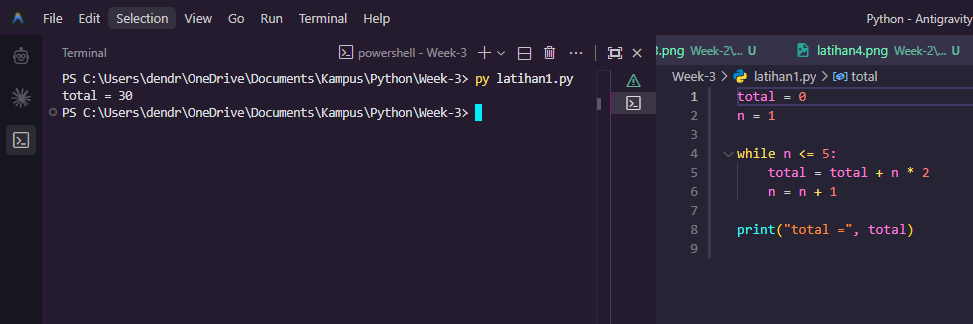
\includegraphics[width=0.85\textwidth]{image/latihan1.png}%
    }{%
        \IfFileExists{image/w3_latihan1.png}{%
            \includegraphics[width=0.85\textwidth]{image/w3_latihan1.png}%
        }{%
            \imageplaceholder{Output Percobaan 1: Penelusuran While dan Trace Table}%
        }%
    }
    \caption{Hasil/Output Percobaan 1: Penelusuran While dan Trace Table}
\end{figure}

\subsubsection{Analisis}
Percobaan 1 membuktikan kegunaan tabel penelusuran (*trace table*) dalam memvalidasi kebenaran semantik kode. Jalannya komputasi dapat dipetakan secara eksak melalui tabel status transisi variabel:
\begin{table}[H]
\centering
\small
\renewcommand{\arraystretch}{1.2}
\begin{tabular}{cccccc}
\toprule
\textbf{Iterasi ke-} & \textbf{Kondisi ($n \le 5$)} & \textbf{Nilai Awal $total$} & \textbf{Ekspresi ($n \times 2$)} & \textbf{Nilai Akhir $total$} & \textbf{Nilai Baru $n$} \\
\midrule
1 & $1 \le 5$ (True) & 0 & $1 \times 2 = 2$ & 2 & 2 \\
2 & $2 \le 5$ (True) & 2 & $2 \times 2 = 4$ & 6 & 3 \\
3 & $3 \le 5$ (True) & 6 & $3 \times 2 = 6$ & 12 & 4 \\
4 & $4 \le 5$ (True) & 12 & $4 \times 2 = 8$ & 20 & 5 \\
5 & $5 \le 5$ (True) & 20 & $5 \times 2 = 10$ & 30 & 6 \\
Terminasi & $6 \le 5$ (False) & 30 & -- & 30 & 6 (Loop Berhenti) \\
\bottomrule
\end{tabular}
\caption{Tabel Penelusuran Transisi State Variabel pada Percobaan 1}
\end{table}
Penelusuran di atas membuktikan bahwa variabel kendali $n$ bertambah secara monotonik sebesar $+1$ pada setiap iterasi. Monotonisitas ini memberikan jaminan terminasi (*termination guarantee*), di mana kondisi $n \le 5$ dipastikan akan bernilai \textit{False} ketika $n = 6$, menghasilkan luaran akhir deterministik sebesar 30.

\subsection{Percobaan 2: Analisis Kesalahan Off-by-One pada Penjumlahan Deret}
\subsubsection{Algoritma}
\begin{enumerate}
    \item Mulai program.
    \item Baca masukan bilangan integer ke dalam variabel \texttt{n}.
    \item Inisialisasi variabel penampung $total = 0$ dan penunjuk nilai $i = 1$.
    \item Uji kondisi perulangan: selama $i \le n$:
    \begin{enumerate}[label=\alph*.]
        \item Tambahkan nilai $i$ ke akumulator: $total = total + i$.
        \item Tambahkan variabel langkah: $i = i + 1$.
    \end{enumerate}
    \item Tampilkan hasil akhir: cetak label dan isi variabel \texttt{total}.
    \item Selesai.
\end{enumerate}

\subsubsection{Hasil / Output}
\begin{figure}[H]
    \centering
    \IfFileExists{image/latihan2.png}{%
        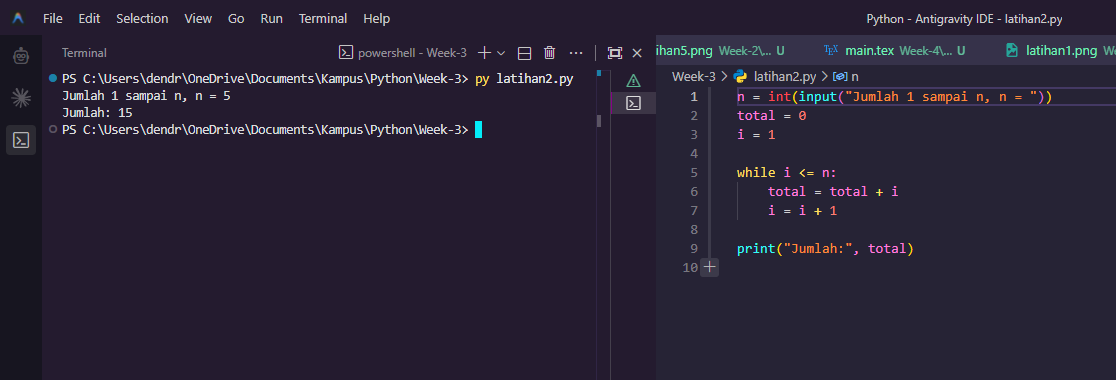
\includegraphics[width=0.85\textwidth]{image/latihan2.png}%
    }{%
        \IfFileExists{image/w3_latihan2.png}{%
            \includegraphics[width=0.85\textwidth]{image/w3_latihan2.png}%
        }{%
            \imageplaceholder{Output Percobaan 2: Pencegahan Off-by-One Deret}%
        }%
    }
    \caption{Hasil/Output Percobaan 2: Pencegahan Off-by-One Deret}
\end{figure}

\subsubsection{Analisis}
Percobaan 2 mendemonstrasikan signifikansi operator batas dalam menghindari galat satu putaran (*off-by-one error*). Secara matematis, jumlah deret bilangan asli pertama didefinisikan oleh rumus Gauss $S_n = \frac{n(n+1)}{2}$. Apabila $n = 5$, nilai teoritis yang diharapkan adalah $\frac{5 \times 6}{2} = 15$.
\begin{itemize}
    \item Jika digunakan kondisi batas ketat $i < n$, perulangan akan berhenti saat $i = 5$, sehingga iterasi ke-5 dilewati dan menghasilkan jumlahan keliru $1+2+3+4 = 10$.
    \item Dengan menggunakan operator relasional inklusif $i \le n$, putaran saat $i = 5$ tetap diproses, menghasilkan nilai yang tepat yaitu 15.
\end{itemize}
Selain itu, program diuji terhadap kondisi batas ekstrem $n = 0$. Karena kondisi $1 \le 0$ langsung dievaluasi menghasilkan \textit{False} sejak awal, blok perulangan langsung diabaikan dan program secara konsisten mencetak nilai $total = 0$ tanpa menyebabkan galat logika maupun *infinite loop*.

\subsection{Percobaan 3: Perulangan Sentinel dan Proteksi Pembagian Nol}
\subsubsection{Algoritma}
\begin{enumerate}
    \item Mulai program.
    \item Inisialisasi $total = 0$ dan $banyak = 0$.
    \item Lakukan *priming read*: baca input integer durasi proses ke variabel \texttt{durasi}.
    \item Jalankan perulangan \texttt{while} selama $durasi \ne -1$:
    \begin{enumerate}[label=\alph*.]
        \item Tambahkan durasi ke total: $total = total + durasi$.
        \item Naikkan pencacah rekaman sah: $banyak = banyak + 1$.
        \item Lakukan *update read*: minta dan baca kembali masukan ke variabel \texttt{durasi}.
    \end{enumerate}
    \item Uji validitas penampung data:
    \begin{enumerate}[label=\alph*.]
        \item Jika $banyak == 0$, cetak string \texttt{"Belum ada data yang dimasukkan."}.
        \item Jika $banyak > 0$, cetak kuantitas data \texttt{banyak} dan rata-rata $\text{round}(total / banyak, 2)$.
    \end{enumerate}
    \item Selesai.
\end{enumerate}

\subsubsection{Hasil / Output}
\begin{figure}[H]
    \centering
    \IfFileExists{image/latihan3.png}{%
        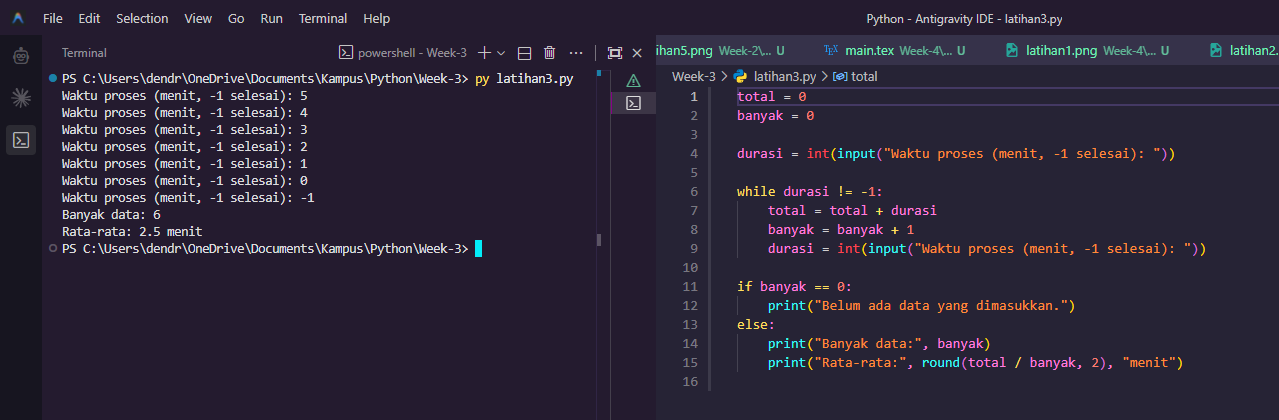
\includegraphics[width=0.85\textwidth]{image/latihan3.png}%
    }{%
        \IfFileExists{image/w3_latihan3.png}{%
            \includegraphics[width=0.85\textwidth]{image/w3_latihan3.png}%
        }{%
            \imageplaceholder{Output Percobaan 3: Sentinel dan Proteksi Zero-Division}%
        }%
    }
    \caption{Hasil/Output Percobaan 3: Sentinel dan Proteksi Zero-Division}
\end{figure}

\subsubsection{Analisis}
Percobaan 3 menyoroti dua pilar penting dalam penanganan data interaktif:
\begin{enumerate}
    \item \textbf{Arsitektur Baca Ganda (\textit{Read-Twice Pattern})}: Dengan meletakkan pembacaan data sebelum loop dan tepat di akhir blok perulangan, nilai penanda ($-1$) dievaluasi langsung pada klausa kondisi \texttt{while durasi != -1}. Ketika pengguna memasukkan $-1$, alur seketika keluar dari perulangan sebelum nilai $-1$ tersebut sempat dijumlahkan ke dalam \texttt{total} atau menaikkan variabel \texttt{banyak}. Hal ini mencegah kontaminasi data statistik.
    \item \textbf{Penjaga Pembagian Nol (\textit{Zero-Division Guard})}: Pada saat program dijalankan dan pengguna langsung memasukkan nilai $-1$, nilai variabel \texttt{banyak} tetap 0. Tanpa adanya struktur percabangan \texttt{if banyak == 0:}, instruksi pembagian $total / banyak$ akan membangkitkan eksepsi fatal \texttt{ZeroDivisionError: division by zero}. Kehadiran percabangan ini memberikan perlindungan komputasi yang membuat aplikasi aman dari penghentian mendadak (*crash*).
\end{enumerate}

\subsection{Percobaan 4: Pola Akumulator dan Pencacah Produksi Harian}
\subsubsection{Algoritma}
\begin{enumerate}
    \item Mulai program.
    \item Inisialisasi konstanta $TARGET = 50$, $HARI = 10$, serta variabel $total = 0$ dan $di\_bawah = 0$.
    \item Jalankan perulangan \texttt{for} dengan variabel \texttt{hari} pada rentang \texttt{range(1, HARI + 1)}:
    \begin{enumerate}[label=\alph*.]
        \item Baca masukan produksi ke variabel \texttt{produksi}.
        \item Jumlahkan ke akumulator: $total = total + produksi$.
        \item Uji ambang batas: jika $produksi < TARGET$, naikkan pencacah $di\_bawah = di\_bawah + 1$.
    \end{enumerate}
    \item Tampilkan nilai akumulator \texttt{total}, rata-rata $total / HARI$, dan nilai pencacah \texttt{di\_bawah}.
    \item Selesai.
\end{enumerate}

\subsubsection{Hasil / Output}
\begin{figure}[H]
    \centering
    \IfFileExists{image/latihan4.png}{%
        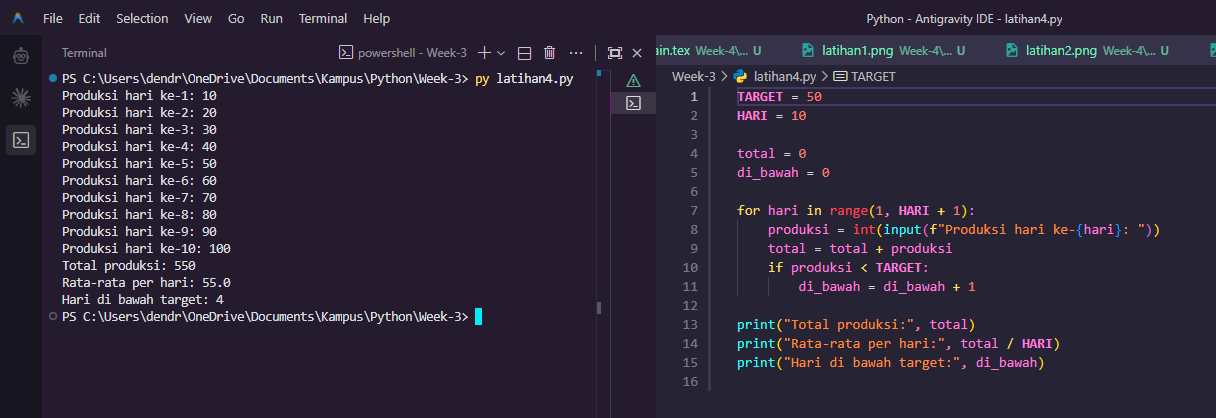
\includegraphics[width=0.85\textwidth]{image/latihan4.png}%
    }{%
        \IfFileExists{image/w3_latihan4.png}{%
            \includegraphics[width=0.85\textwidth]{image/w3_latihan4.png}%
        }{%
            \imageplaceholder{Output Percobaan 4: Akumulator dan Pencacah Produksi}%
        }%
    }
    \caption{Hasil/Output Percobaan 4: Akumulator dan Pencacah Produksi}
\end{figure}

\subsubsection{Analisis}
Percobaan 4 menerapkan pemisahan peran variabel dalam satu perulangan tunggal (*dual-pattern iteration*). Variabel \texttt{total} berfungsi murni sebagai akumulator yang bersifat aditif terhadap seluruh rekaman data masukan tanpa terkecuali. Sebaliknya, variabel \texttt{di\_bawah} berfungsi sebagai pencacah selektif (*conditional counter*) yang hanya bertambah ketika kondisi relasional $produksi < 50$ terpenuhi.

Perhitungan rata-rata harian memanfaatkan sifat deterministik dari konstanta $HARI = 10$. Karena jumlah hari telah dipastikan secara konstan bernilai 10, operasi pembagian $total / HARI$ tidak rentan terhadap galat pembagian dengan nol. Hal ini mencerminkan struktur kendali terhitung (*count-controlled loop*) yang tepat untuk data yang memiliki batas periode definitif.

\subsection{Percobaan 5: Pola Penyaringan Produksi Terhadap Target}
\subsubsection{Algoritma}
\begin{enumerate}
    \item Mulai program.
    \item Tetapkan konstanta $TARGET = 50$, durasi $HARI = 10$, akumulator $total\_lolos = 0$, dan pencacah $banyak\_lolos = 0$.
    \item Jalankan perulangan \texttt{for} untuk \texttt{hari} dari 1 hingga $HARI$:
    \begin{enumerate}[label=\alph*.]
        \item Baca masukan produksi ke variabel \texttt{produksi}.
        \item Uji kondisi penyaring: periksa apakah $produksi \ge TARGET$.
        \item Jika benar (\textit{True}): perbarui $total\_lolos = total\_lolos + produksi$ dan $banyak\_lolos = banyak\_lolos + 1$.
    \end{enumerate}
    \item Evaluasi hasil penyaringan:
    \begin{enumerate}[label=\alph*.]
        \item Jika $banyak\_lolos == 0$: tampilkan pesan \texttt{"Tidak ada hari yang mencapai target."}.
        \item Selain itu: hitung nilai rata-rata kelompok lolos $rata = \text{round}(total\_lolos / banyak\_lolos, 2)$, lalu cetak nilai \texttt{banyak\_lolos}, \texttt{total\_lolos}, dan \texttt{rata}.
    \end{enumerate}
    \item Selesai.
\end{enumerate}

\subsubsection{Hasil / Output}
\begin{figure}[H]
    \centering
    \IfFileExists{image/latihan5.png}{%
        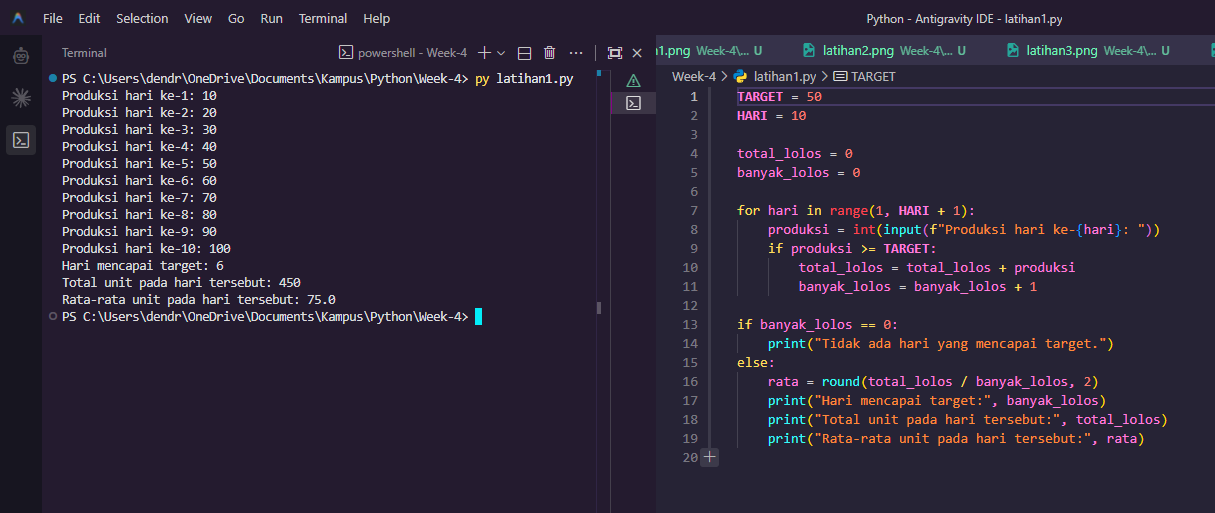
\includegraphics[width=0.85\textwidth]{image/latihan5.png}%
    }{%
        \IfFileExists{image/w4_latihan1.png}{%
            \includegraphics[width=0.85\textwidth]{image/w4_latihan1.png}%
        }{%
            \imageplaceholder{Output Percobaan 5: Pola Penyaringan Produksi}%
        }%
    }
    \caption{Hasil/Output Percobaan 5: Pola Penyaringan Produksi}
\end{figure}

\subsubsection{Analisis}
Percobaan 5 memperdalam penerapan pola penyaringan (*filtering pattern*). Berbeda dengan percobaan sebelumnya di mana seluruh data diakumulasikan, pada pola ini akumulator \texttt{total\_lolos} dan pencacah \texttt{banyak\_lolos} berada di dalam blok kondisi seleksi \texttt{if produksi >= TARGET:}. Akibatnya, elemen data yang bernilai di bawah ambang target secara efektif diabaikan dari himpunan perhitungan.

Implikasi krusial dari pola penyaringan adalah ukuran himpunan hasil saring yang bersifat variabel ($0 \le banyak\_lolos \le 10$). Apabila dalam suatu pengujian seluruh masukan produksi harian bernilai di bawah 50, maka \texttt{banyak\_lolos} akan bernilai 0. Oleh karena itu, penyematan blok proteksi \texttt{if banyak\_lolos == 0:} menjadi mutlak diperlukan sebelum operasi pembagian rata-rata dilakukan guna mencegah kegagalan runtime \texttt{ZeroDivisionError}.

\subsection{Percobaan 6: Pelacakan Nilai Ekstrem dan Jebakan Inisialisasi}
\subsubsection{Algoritma}
\begin{enumerate}
    \item Mulai program.
    \item Tetapkan penanda nilai awal aman: $tertinggi = \text{None}$ dan $bulan\_tertinggi = \text{None}$.
    \item Jalankan perulangan \texttt{for} dengan variabel \texttt{bulan} pada rentang \texttt{range(1, 7)}:
    \begin{enumerate}[label=\alph*.]
        \item Baca nilai laba bulanan ke variabel integer \texttt{laba}.
        \item Uji kondisi nilai ekstrem: periksa apakah $tertinggi \text{ is None}$ atau $laba > tertinggi$.
        \item Jika benar (\textit{True}): perbarui nilai $tertinggi = laba$ dan simpan indeks $bulan\_tertinggi = bulan$.
    \end{enumerate}
    \item Cetak luaran dengan format f-string yang memuat nilai \texttt{tertinggi} dan nomor \texttt{bulan\_tertinggi}.
    \item Selesai.
\end{enumerate}

\subsubsection{Hasil / Output}
\begin{figure}[H]
    \centering
    \IfFileExists{image/latihan6.png}{%
        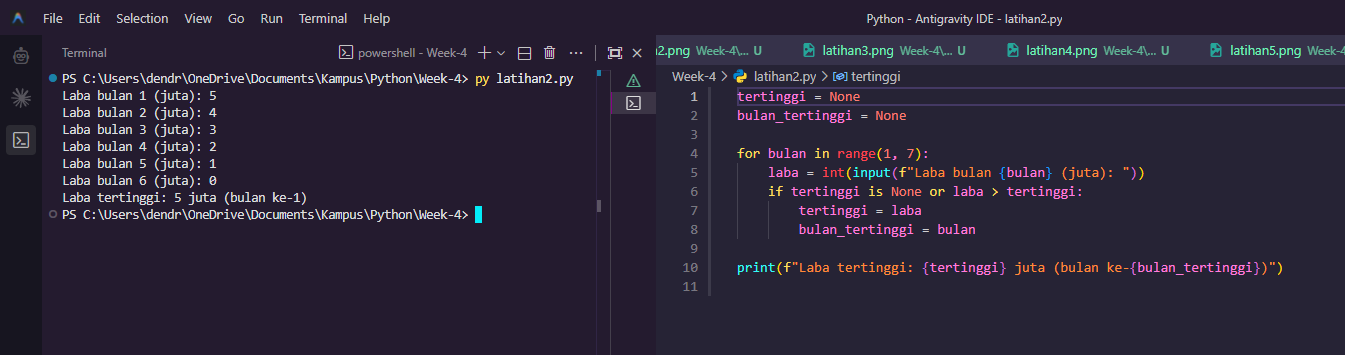
\includegraphics[width=0.85\textwidth]{image/latihan6.png}%
    }{%
        \IfFileExists{image/w4_latihan2.png}{%
            \includegraphics[width=0.85\textwidth]{image/w4_latihan2.png}%
        }{%
            \imageplaceholder{Output Percobaan 6: Nilai Ekstrem dan Inisialisasi None}%
        }%
    }
    \caption{Hasil/Output Percobaan 6: Nilai Ekstrem dan Inisialisasi None}
\end{figure}

\subsubsection{Analisis}
Percobaan 6 memberikan pembuktian teoritis terhadap jebakan inisialisasi nilai ekstrem (*initial value pitfall*). Praktik umum yang keliru adalah menetapkan nilai awal $tertinggi = 0$. Misalkan kinerja keuangan suatu unit usaha selama 6 bulan berturut-turut mengalami kerugian: $-10$, $-5$, $-15$, $-8$, $-20$, $-12$.
\begin{itemize}
    \item Jika diinisialisasi dengan $tertinggi = 0$, maka perbandingan $-10 > 0$, $-5 > 0$, dan seterusnya akan selalu bernilai \textit{False}. Program akan secara salah menyimpulkan bahwa laba tertinggi adalah $0$, padahal angka 0 tidak pernah ada di dalam data dan kinerja terbaik riil adalah $-5$ juta pada bulan ke-2.
    \item Dengan memanfaatkan penanda \texttt{None}, kondisi $tertinggi \text{ is None}$ pada bulan pertama otomatis bernilai \textit{True}. Akibatnya, nilai masukan pertama ($-10$) langsung diangkat menjadi basis pembanding riil. Pada bulan kedua, nilai $-5$ berhasil menggeser $-10$ karena $-5 > -10$, sehingga program secara presisi menetapkan laba tertinggi $-5$ juta pada bulan ke-2.
\end{itemize}
Penyimpanan variabel simultan $bulan\_tertinggi = bulan$ membuktikan efektivitas pelacakan indeks kejadian temporal bersamaan dengan nilai ekstrem skalar.

\subsection{Percobaan 7: Pengelompokan Masalah Suhu Mesin}
\subsubsection{Algoritma}
\begin{enumerate}
    \item Mulai program.
    \item Inisialisasi variabel tiga kelompok masalah: $tertinggi = \text{None}$, $urutan\_tertinggi = \text{None}$, $banyak\_diatas\_80 = 0$, dan $total\_diatas\_80 = 0$.
    \item Lakukan iterasi terhitung \texttt{for} dengan variabel $i$ dari 1 sampai 8:
    \begin{enumerate}[label=\alph*.]
        \item Baca masukan pembacaan suhu sensor ke variabel \texttt{suhu}.
        \item Penanganan Sub-masalah 1: jika $tertinggi \text{ is None}$ atau $suhu > tertinggi$, perbarui $tertinggi = suhu$ dan $urutan\_tertinggi = i$.
        \item Penanganan Sub-masalah 2 dan 3: jika $suhu > 80$, perbarui $banyak\_diatas\_80 = banyak\_diatas\_80 + 1$ dan $total\_diatas\_80 = total\_diatas\_80 + suhu$.
    \end{enumerate}
    \item Tampilkan nilai suhu tertinggi beserta nomor urut kejadiannya.
    \item Evaluasi luaran suhu kritis: jika $banyak\_diatas\_80 == 0$, cetak pesan ketiadaan data kritis. Jika ada, hitung rata-rata suhu kritis dan tampilkan dengan pemformatan presisi desimal \texttt{:.2f}.
    \item Selesai.
\end{enumerate}

\subsubsection{Hasil / Output}
\begin{figure}[H]
    \centering
    \IfFileExists{image/latihan7.png}{%
        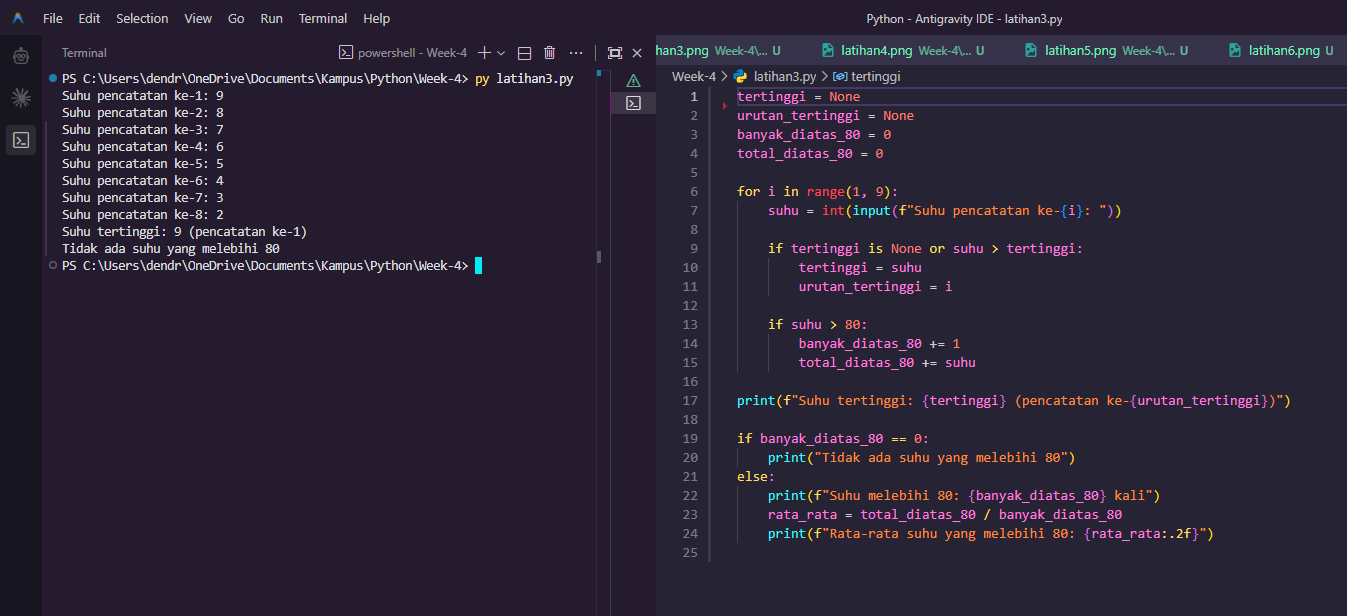
\includegraphics[width=0.85\textwidth]{image/latihan7.png}%
    }{%
        \IfFileExists{image/w4_latihan3.png}{%
            \includegraphics[width=0.85\textwidth]{image/w4_latihan3.png}%
        }{%
            \imageplaceholder{Output Percobaan 7: Problem Grouping Suhu Mesin}%
        }%
    }
    \caption{Hasil/Output Percobaan 7: Problem Grouping Suhu Mesin}
\end{figure}

\subsubsection{Analisis}
Percobaan 7 mengilustrasikan penerapan paradigma dekomposisi masalah dan pengelompokan pola (*problem grouping*). Permasalahan analitik yang melibatkan beberapa kebutuhan output tidak diselesaikan dengan menulis beberapa loop terpisah, melainkan diintegrasikan ke dalam satu siklus iterasi yang terstruktur rapi.

Pengelompokan ini memisahkan dua domain logika:
\begin{itemize}
    \item Domain global (pelacakan ekstrem menyeluruh): mengevaluasi setiap titik data sensor untuk mencari suhu puncak.
    \item Domain lokal bersyarat (penyaringan ambang kritis $> 80$): mengisolasi anomali termal untuk menghitung frekuensi bahaya dan magnitudo rata-rata temperatur tinggi.
\end{itemize}
Pemisahan variabel akumulator khusus (\texttt{total\_diatas\_80}) dan pencacah khusus (\texttt{banyak\_diatas\_80}) memastikan tidak ada interferensi antar parameter statistik, menghasilkan performa algoritma yang efisien dengan kompleksitas waktu linear $\mathcal{O}(n)$ dan kompleksitas memori konstan $\mathcal{O}(1)$.

\subsection{Percobaan 8: Studi Kasus Rekapitulasi Produksi Lini Perakitan}
\subsubsection{Algoritma}
\begin{enumerate}
    \item Mulai program.
    \item Tetapkan parameter sistem: $TARGET = 100$ dan $PENANDA = -1$.
    \item Inisialisasi variabel pelacak: $banyak\_hari = 0$, $total\_produksi = 0$, $hari\_target = 0$, $total\_target = 0$, serta $tertinggi = hari\_tertinggi = terendah = hari\_terendah = \text{None}$.
    \item Lakukan *priming read*: baca produksi hari pertama ke variabel \texttt{produksi}.
    \item Lakukan perulangan \texttt{while} selama $produksi \ne PENANDA$:
    \begin{enumerate}[label=\alph*.]
        \item Naikkan kuantitas hari: $banyak\_hari = banyak\_hari + 1$ dan jumlahkan $total\_produksi = total\_produksi + produksi$.
        \item Inisialisasi rekaman pertama: jika $banyak\_hari == 1$, tetapkan $tertinggi = terendah = produksi$ dan $hari\_tertinggi = hari\_terendah = 1$.
        \item Pembaruan ekstrem rekaman lanjutan ($banyak\_hari > 1$):
        \begin{itemize}
            \item Jika $produksi > tertinggi$, perbarui $tertinggi = produksi$ dan $hari\_tertinggi = banyak\_hari$.
            \item Jika $produksi < terendah$, perbarui $terendah = produksi$ dan $hari\_terendah = banyak\_hari$.
        \end{itemize}
        \item Penyaringan hari target: jika $produksi \ge TARGET$, perbarui $hari\_target = hari\_target + 1$ dan $total\_target = total\_target + produksi$.
        \item Lakukan *update read*: baca produksi hari berikutnya ke variabel \texttt{produksi}.
    \end{enumerate}
    \item Periksa integritas data: jika $banyak\_hari == 0$, tampilkan notifikasi \texttt{"Belum ada data produksi."}.
    \item Jika ada data: hitung rata-rata keseluruhan $rata\_rata = total\_produksi / banyak\_hari$ dan tampilkan ringkasan lengkap. Jika $hari\_target > 0$, hitung dan cetak rata-rata khusus hari target $total\_target / hari\_target$.
    \item Selesai.
\end{enumerate}

\subsubsection{Hasil / Output}
\begin{figure}[H]
    \centering
    \IfFileExists{image/studi_kasus.png}{%
        \includegraphics[width=0.85\textwidth]{image/studi_kasus.png}%
    }{%
        \IfFileExists{image/latihan8.png}{%
            \includegraphics[width=0.85\textwidth]{image/latihan8.png}%
        }{%
            \imageplaceholder{Output Percobaan 8: Studi Kasus Lini Perakitan}%
        }%
    }
    \caption{Hasil/Output Percobaan 8: Studi Kasus Lini Perakitan}
\end{figure}

\subsubsection{Analisis}
Studi kasus ini merupakan sintesis komprehensif seluruh materi Modul 3 dan 4. Terdapat tiga keunggulan algoritma yang diimplementasikan:
\begin{enumerate}
    \item \textbf{Inisialisasi Rekaman Pertama (*First-Record Initialization*)}: Pada saat $banyak\_hari == 1$, nilai produksi hari pertama langsung dijadikan nilai awal untuk $tertinggi$ dan $terendah$. Pendekatan ini merupakan alternatif elegan pengganti inisialisasi \texttt{None}, yang secara mutlak menjamin rentang pencarian ekstrem berada pada domain data valid.
    \item \textbf{Pemutus Seri Hari Terawal (*Earliest Tie-Breaker*)}: Penggunaan operator perbandingan ketat ($>$ dan $<$) memastikan bahwa apabila terdapat dua hari kerja yang menghasilkan volume produksi puncak kembar (misal hari ke-2 dan hari ke-5 sama-sama memproduksi 150 unit), maka indeks hari yang dipertahankan adalah hari kejadian pertama (hari ke-2). Sebaliknya, jika digunakan operator $\ge$, indeks akan tertimpa oleh kejadian terakhir. Karakteristik ini penting untuk audit logistik operasional.
    \item \textbf{Agregasi Ganda dengan Proteksi Berlapis}: Program mampu menyajikan perbandingan antara rata-rata produksi keseluruhan dan rata-rata performa khusus hari target secara dinamis. Proteksi pembagian nol diterapkan secara independen pada level transaksi umum ($banyak\_hari == 0$) dan level transaksi target ($hari\_target == 0$). Hal ini mencerminkan prinsip rancang bangun kode standar industri yang andal dan tahan banting.
\end{enumerate}

% ============================================================
% KESIMPULAN
% ============================================================
\section{KESIMPULAN}
Berdasarkan serangkaian perancangan, verifikasi, dan analisis komputasi pada Modul Praktikum 3 dan 4, dapat ditarik kesimpulan fundamental sebagai berikut:
\begin{enumerate}
    \item Pemanfaatan tabel penelusuran (*trace table*) merupakan instrumen verifikasi krusial untuk membuktikan jaminan terminasi (*termination guarantee*) dan memastikan variabel kendali bertransisi secara konsisten menuju kondisi terminasi perulangan.
    \item Kesalahan satu putaran (*off-by-one error*) timbul akibat ketidaktelitian pemilihan operator relasional batas ($\le$ versus $<$), dan dapat diantisipasi melalui pengujian nilai batas inklusif serta verifikasi pada kasus ekstrem nol ($n = 0$) dan satu ($n = 1$).
    \item Pola perulangan berpenanda (*sentinel*) mutlak membutuhkan skema pembacaan ganda (*read-twice pattern*), yaitu pembacaan inisiasi sebelum perulangan dan pembacaan akhir siklus, guna menjamin nilai penanda tidak mengontaminasi akumulator atau pencacah data.
    \item Pola penyaringan (*filtering pattern*) memisahkan data agregat berdasarkan ambang batas (*threshold*), dan secara inheren menuntut keberadaan proteksi kondisi (*zero-division guard*) sebelum operasi pembagian rata-rata dieksekusi.
    \item Menginisialisasi nilai ekstrem dengan angka nol ($tertinggi = 0$) merupakan jebakan logika fatal (*initial value pitfall*) pada domain data riil atau negatif. Pola inisialisasi berbasis penanda \texttt{None} atau inisialisasi rekaman pertama (*first-record initialization*) menjamin kebenaran komputasi nilai ekstrem secara universal.
    \item Dekomposisi masalah (*problem grouping*) memungkinkan integrasi berbagai pola komputasi (akumulasi umum, penyaringan kondisional, serta pelacakan indeks temporal ekstrem) ke dalam satu lintasan perulangan linear berkinerja tinggi ($\mathcal{O}(n)$).
\end{enumerate}

% ============================================================
% DAFTAR PUSTAKA
% ============================================================
\section{DAFTAR PUSTAKA}

\begin{enumerate}
    \item Tim Dosen Algoritma dan Pemrograman. (2025). \textit{Modul Praktikum 3 \& 4: Pola Perulangan: Penelusuran, Penanda, dan Pengolahan Data}. Program Studi S1 Sistem Informasi, Fakultas Rekayasa Industri, Telkom University Surabaya.

    \item Python Software Foundation. (2024). \textit{The Python Tutorial: More Control Flow Tools (Release 3.12)}. Diakses dari \url{https://docs.python.org/3/tutorial/controlflow.html}.

    \item McConnell, S. (2004). \textit{Code Complete: A Practical Handbook of Software Construction (2nd Edition)}. Microsoft Press.

    \item Sedgewick, R., \& Wayne, K. (2016). \textit{Computer Science: An Interdisciplinary Approach}. Addison-Wesley Professional.
\end{enumerate}

\end{document}
